%mark = star, diamond, square, otimes
%\documentclass{article}
%\usepackage{pgfplots}
%\usepackage[justification=centering]{caption}
%\pgfplotsset{compat=newest}
%\begin{document}
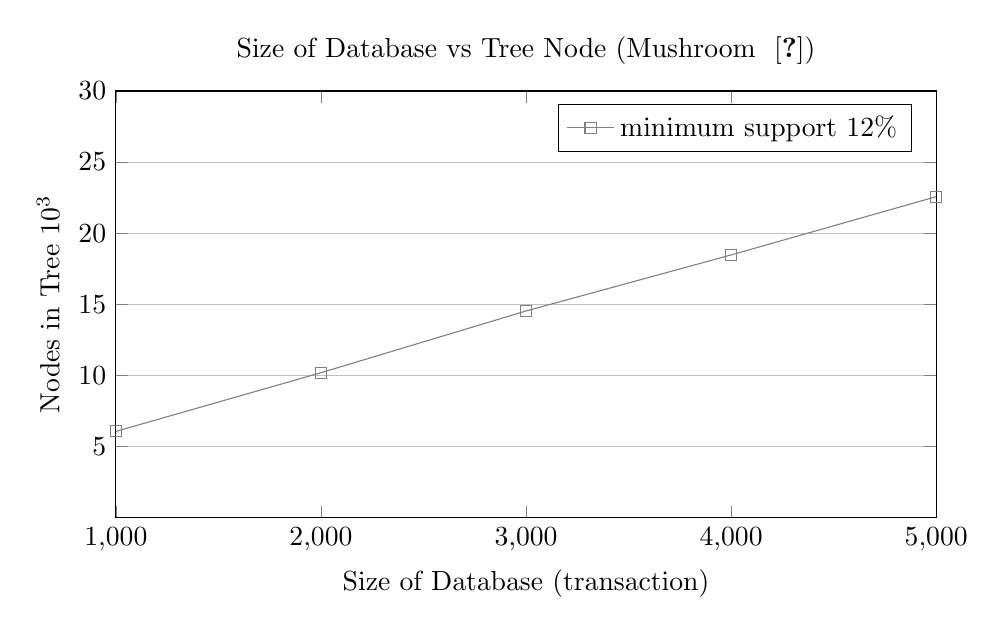
\begin{tikzpicture}
\begin{axis}[
	title={Size of Database vs Tree Node (Mushroom ~\cite{dataset})},
	width=12cm,
	height=7cm,
	xlabel={Size of Database (transaction)},
    ylabel={Nodes in Tree $10^3$},
    xmin=1000, xmax=5000,
    ymin=0, ymax=30,
    xtick={1000,2000,3000,4000,5000},
    ytick={5,10,15,20,25,30},
    legend pos=north east,
    ymajorgrids=true,
    grid style={line width=.2pt,draw=gray!50},
]
 
\addplot[
    solid,color=gray, every mark/.append style={solid, fill=gray}, mark=square
    ]
    coordinates {
			(1000,6.061 )
			(2000,10.187)
			(3000,14.528)
			(4000,18.469)
			(5000,22.566)


	};
    \addlegendentry{minimum support 12\%}

\end{axis}
\end{tikzpicture}
%\end{document}